
\chapter{Technical Background}	\label{chap:background}
\section{General processing chain}\label{sec:tech_general}
%audio - pre-processing - feat. extraction - machine learning
% unseen audio - pre-processing - feat. extraction  - run through model - result

The general procedure for the tasks in this work is shown in figures \ref{fig:process_training} and \ref{fig:process_classification}. Using data sets of audio (speech or singing) and matching annotations, models are trained as outlined in figure \ref{fig:process_training}. Then, these models are used to classify unseen audio data in order to generate annotations for them.\\
In detail, the necessary steps are:
\begin{description}
\item[Pre-processing] For the tasks in this work, pre-processing of the audio data is relatively straightforward and consists of normalization of the signal and averaging to a mono channel. Additionally, the audio is usually downsampled to $16kHz$ because this is the lowest sampling frequency in most of the data sets, and downsampling is necessary for compatibility (more detail on the data sets is given in chapter \ref{chap:datasets}).
\item[Feature extraction] The audio signal contains a lot of data that is redundant and irrelevant to the tasks. For this reason, many types of so-called feature representations were developed over the years. The features employed in this work are described in the next section.
\item[Model training] Using both the audio features and the available annotations, models are trained with machine learning algorithms to gain an implicit understanding of the requested annotations (i.e. classes). In this work, only supervised learning was employed. The machine learning methods are described in section \ref{sec:tech_ml}.
\item[Classification] The trained models can then be used on features extracted from unseen audio data to obtain their annotations (= classes).
\item[Post-processing] In many tasks, the classification results are not used directly, but processed further. In tasks like alignment and retrieval, for example, phoneme probabilities are matched with symbolic phoneme annotations. In these cases, distance calculation methods as described in section \ref{sec:tech_distances} are required.
\end{description}
Implementation of these steps for the actual tasks is described in section \ref{sec:tech_systems}.

\begin{figure}
	\begin{center}
		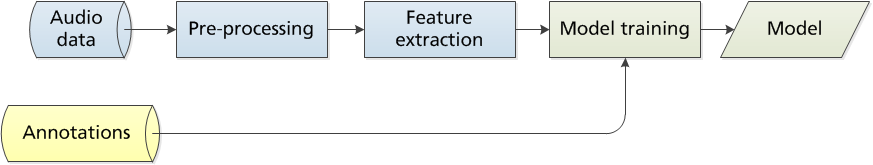
\includegraphics[width=1\textwidth]{images/process_training.png}
		\caption{Schematic of the training procedure of the considered tasks.}
		\label{fig:process_training}
	\end{center}
\end{figure}
\begin{figure}
	\begin{center}
		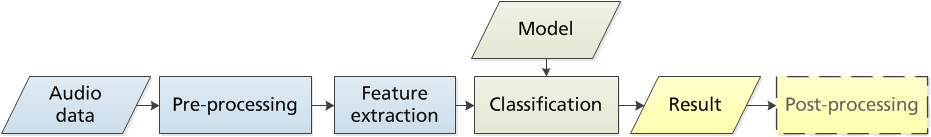
\includegraphics[width=1\textwidth]{images/process_classification}
		\caption{Schematic of the classification procedure of the considered tasks (the model is the one created during training - see figure \ref{fig:process_training}).}
		\label{fig:process_classification}
	\end{center}
\end{figure}

\section{Audio features}
%mfcc, sdc, (rasta-)plp, trap; mention filterbank feats...?
%TODO: write intro
This section describes the various audio features used througout this work. As one of the most successful features in ASR, Mel-Frequency Cepstral Coefficients (MFCCs) were used in all tasks, in some of them as the only feature. Shifted Delta Cepstrum (SDC) features, Perceptual Linear Prediction (PLP) features, and TempoRAl Patterns (TRAPs) were used in language identification. All features were extracted with a time resolution of 10ms, with window sizes of 20 to 25ms.
\subsection{Mel-Frequency Cepstral Coefficients (MFCCs)} 
%!
MFCCs are among the most frequently used audio features in speech recognition and Music Information Retrieval \cite{sahidullah}\cite{meinard_retrieval}. They were first introduced in 1976 by Mermelstein and Davis \cite{mermelstein}\cite{davis_mermelstein} based on previous experiments by Bridle and Brown \cite{bridle_brown}.\\

The basic idea behind MFCCs comes from experiments in human auditory perception. Audio signals are transformed into a representation that is based on human perceptual sensitivities. This is done by taking the Short-Term Fourier Transform (STFT) of an audio signal and then mapping the resulting spectrum from a linear frequency scale onto a Mel scale. Then, the Discrete Cosine Transform (DCT) of the resulting log energies is calculated along the frequency axis to decorrelate the spectral band signals. The result is a representation of the various frequencies within the spectrum (i.e. the cepstrum), which can be interpreted as ranging from the spectral envelope to the more fine-grained components. In theory, this makes the result largely independent of the absolute frequencies (i.e. the pitch), but representative of the perceptual content (e.g. phonemes). One point of criticism, however, is the lack of interpretability of the MFC coefficients.\\

In detail, the calculation is performed as follows:
\begin{description}
\item[1. Short-term Fourier transform (STFT)] After cutting a signal $x$ into frames (e.g. of 10ms duration) and windowing it (e.g. with a Hamming window), the Discrete Fourier Transform (DFT) is calculated for each time frame:
\begin{equation}
X(k) = \sum_{n=0}^{N-1} x(n)h(n)e^{-j 2\pi kn/N} ,  k = 0,1,...,N-1
\end{equation}
where $h(n)$ is the window and $N$ is the DFT length. For the further calculations, only the power spectrum is used:
%???
\begin{equation}
P_i(k) = \frac{1}{N} \mid S_i(k) \mid ^2
\end{equation}

\item[2. Mel-spectrum calculation] The resulting energies are mapped from the linear frequency scale to a perceptually motivated Mel scale. This is done by convolving the spectrum with a set of $M$ triangular Mel-spaced filters $H_i(k)$, such as the ones shown in figure \ref{fig:mel_filterbanks}. Furthermore, the resulting energy outputs are logarithmized:
\begin{equation}
X_i = \log_{10} \left( \sum_{k=0}^{N-1} \mid X(k) \mid \cdot H_i(k) \right), i=1,2,...,M
\end{equation}

\item[3. Discrete Cosine Transform (DCT)] Finally, the Mel-scale spectrum is transformed with a DCT, resulting in the so-called cepstrum:
\begin{equation}
C_j = \sum_{i=1}^M X_i \cdot \cos \left( j \cdot (i-1/2) \cdot \frac{\pi}{M} \right), j=1,2,...,J 
%j \dot (i-1/2) \dot \frac{\pi}{M}
\end{equation}
The $J$ MFC coefficients are retained as features. The 0th coefficient can be interpreted as the power over all frequency bands, and the 1st coefficient as the global energy balance between low and high frequencies \cite{oshaughnessy}.

\end{description}

In this work, 13 coefficients including the 0th coefficient are extracted, with the exception of language identification, where 20 coefficients are used. In addition, deltas and double-deltas are calculated to capture information about the feature's trajectory:
\begin{equation}
\Delta(C(n)) = C(n) - C(n-1) 
\end{equation}
\begin{equation}
\Delta\Delta(C(n)) = \Delta(C(n)) - \Delta(C(n-1))
\end{equation}

\begin{figure}
	\begin{center}
		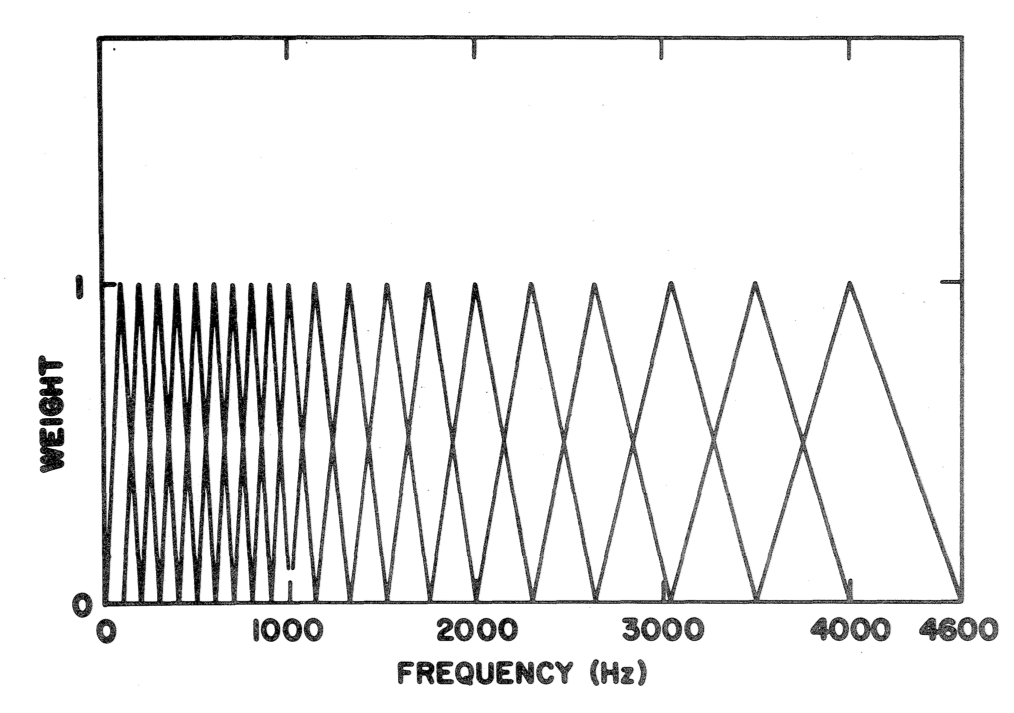
\includegraphics[width=0.6\textwidth]{images/mel_filterbanks.png}
		\caption{Example of a Mel filterbank. \cite{davis_mermelstein}}
		\label{fig:mel_filterbanks}
	\end{center}
\end{figure}



\subsection{Shifted Delta Cepstrum (SDCs)} 
Shifted Delta Cepstrum features were first described in \cite{bielefeld} and have since been successfully used for speaker verification and language identification tasks on speech data \cite{torres} \cite{campbell} \cite{allen}. They are calculated on MFCC vectors and take their temporal evolution into account. This has been shown to improve recognition results because speech and singing signals are defined by their temporal contexts. Their configuration is described by the four parameters $N-d-P-k$, where $N$ is the number of cepstral coefficients for each frame, $d$ is the time context (in frames) for the delta calculation, $k$ is the number of delta blocks to use, and $P$ is the shift between consecutive blocks. The delta cepstrals are then calculated as:
\begin{equation}
\Delta c(t) = c(t+iP+d)+c(t+iP-d), 0<=i<=k
\end{equation}
with $c \in [0, N-1]$ as the previously extracted cepstral coefficients. The resulting $k$ delta cepstrals for each frame are concatenated to form a single SDC vector of the length $kN$. In this work, the common parameter combination $N=7, d=1, P=3, k=7$ was used. The calculation is visualized in figure \ref{fig:sdc_example}.

\begin{figure}
	\begin{center}
		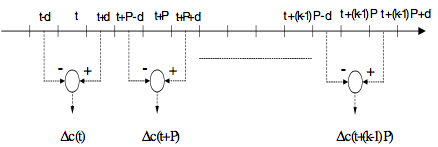
\includegraphics[width=0.8\textwidth]{images/sdc_example.png}
		\caption{The SDC calculation at frame $t$. \cite{torres}}
		\label{fig:sdc_example}
	\end{center}
\end{figure}

%TODO: perceptive or perceptual??
\subsection{Perceptive Linear Predictive features (PLPs)} 
PLP features, first introduced in \cite{hermansky90}, are also among the most frequently used features in speech processing, next to MFCCs. They are based on the idea to use knowledge about human perception to emphasize important speech information in spectra while minimizing the differences between speakers.\\

\begin{figure}
	\begin{center}
		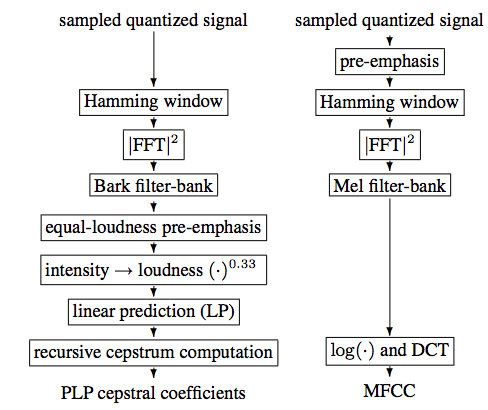
\includegraphics[width=0.8\textwidth]{images/comp_mfcc_plp.png}
		\caption{Comparison of the processing steps in MFCC (left) and PLP (right) calculation. \cite{hoenig}}
		\label{fig:comp_mfcc_plp}
	\end{center}
\end{figure}
In principle, these ideas are related to those that MFCCs are based on, but knowledge about human perception is integrated more extensively. A comparison of the steps of both algorithms is given in figure \ref{fig:comp_mfcc_plp}. For PLP computation, these steps are as follows:
\begin{description}
\item[1. Short-term Fourier transform] As in MFCC extraction, the signal $x$ is segmented into frames, which are then windowed, and the STFT is calculated for each of them. The power spectrum is $X$ is used for further processing.
\item[2. Bark-spectrum calculation] Similar to the Mel-frequency transformation step, the resulting energies $X$ are mapped to a Bark frequency scale, which is also perceptually motivated (resulting in Bark-scaled energies $X_i$). As described in \cite{woodland}�and \cite{hoenig}, there is no necessity for the particular use of a Bark scale, but it is employed for historic reasons. A comparison of the filters of which Mel  and Bark filterbanks are composed is shown in figure \ref{fig:comp_filterbanks}. Furthermore, the coefficients are logarithmized.
\item[3. Equal loudness pre-emphasis] The filterbank coefficients are weighted with an equal-loudness curve $E(f)$ which simulates the varying sensitivities of human hearing across the frequency range. Figure \ref{fig:eq_loudness} displays such a curve; Makhoul and Cosell presented a numerical approximation \cite{makhoul}. (As mentioned in figure \ref{fig:comp_mfcc_plp}, such a pre-emphasis is sometimes performed as the first step of MFCC calculation as well). This is computed as
\begin{equation}
\Xi(f) = X_i(f) \cdot E(f)
\end{equation}
\item[4. Intensity - loudness conversion] This steps integrates knowledge about the relationship between the intensity of the signal and its perceived loudness. According to the power law of hearing \cite{stevens}, this relation can be approximated as a cubic root compression:
\begin{equation}
\Phi(f)  = \Xi(f)^{0.33}
\end{equation}
\item[5. Autoregressive modeling] An inverse DFT is then applied to the computed loudness signal to obtain an auto-correlation function. Then, the actual linear prediction is implemented with an all-pole model as described in \cite{makhoul2}. Levinson-Durbin recursion is employed to compute the final PLP coefficients from the auto-correlation function.
\end{description}
\begin{figure}
	\begin{center}
		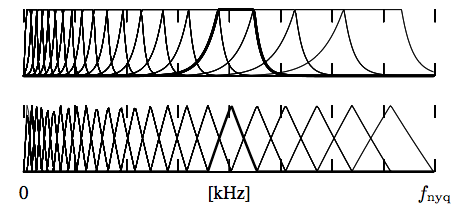
\includegraphics[width=0.7\textwidth]{images/filterbanks_mfcc_plp.png}
		\caption{Mel-scale (top) and Bark-scale filterbank. \cite{hoenig}}
		\label{fig:comp_filterbanks}
	\end{center}
\end{figure}
\begin{figure}
	\begin{center}
		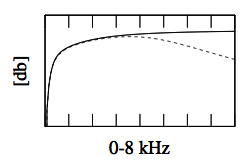
\includegraphics[width=0.4\textwidth]{images/eq_loudness.png}
		\caption{Perceptually motivated equal-loudness weighting function. (The dashed function is used for signals with a Nyquist frequency $>5kHz$). \cite{hoenig}}
		\label{fig:eq_loudness}
	\end{center}
\end{figure}

Later, RASTA filtering was introduced as a step between the Bark-spectrum calculation and the equal loudness pre-emphasis (i.e. steps 2 and 3) \cite{rasta_plp}. This is essentially a bandpass filtering in the log-spectral domain that serves to suppress the slow-changing components of the signal, which are commonly rooted in the transmission channel rather than the content. The filter is defined as
\begin{equation}
H(z) = 0.1 \frac{2+z^{-1}-z^{-3}-2z^{-4}}{z^{-4}\cdot (1-0.98z^{-1})}
\end{equation}\\

In this work, model orders of 13 and 36 are used. Deltas and double-deltas between frames are also calculated, and PLPs are tested with and without RASTA pre-processing.


\subsection{TempoRal Patterns (TRAP)} 
TRAPs were developed by Hermansky \cite{traps1} \cite{traps2} and have also been used successfully in a number of speech recognition tasks. In contrast to MFCCs and PLPs, which, apart from delta calculation, only consider a single spectral frame at a time, TRAPs take the spectral development over time into account. This is visualized in figure \ref{fig:trap_temporal}. To demonstrate the feature's suitability for phoneme classification, examples of mean TRAPs for various phonemes in the 5th critical band are shown in figure \ref{fig:phoneme_traps}.\\

In \cite{matejka}, a slightly modified method is presented. An overview of the steps necessary for this version of TRAP calculation is given in figure \ref{fig:traps}. In detail, these are:
\begin{description}
\item[1. Grouping into spectral bands]  Spectral band signals are extracted from the signal with a triangular Mel-scale filterbank, such as the one presented in figure \ref{fig:mel_filterbanks}. The log-energy of each band is used for further processing.
\item[2. Normalization and windowing] Each band's trajectory is normalized and windowed with relatively long windows (e.g. Hamming windows with a temporal context of 200 to 1000ms) to obtain a representation of the temporal development.
\item[3. DCT decorrelation] A DCT is applied to each frame to decorrelate its coefficients and reduce dimensionality. The vectors for each critical band are concatenated. (In classical TRAP calculation, separate classifiers would be trained for each band in this step).
\item[4. Model training] In classical TRAP calculation, the resulting band coefficients are now used to train a Multilayer Perceptron with a single hidden layer to obtain phoneme probabilities \cite{matejka}. However, as suggested in \cite{jens}, the feature values extracted so far can also be used to train other models, or even be combined with other features beforehand. In \cite{robust_asr}, the authors suggest that a combination with MFCCs works particularly well as these two features cover different sets of characteristics: MFCCs are better at capturing the spectral content, while TRAPs model the temporal progressions better.
\end{description}

In this work, the coefficient vector is used directly as a feature to train various models. 8 linear spectral bands were extracted with a time context of 20 frames (corresponding to 200ms), and the first 8 DCT coefficients were kept.

\begin{figure}
 \centerline{\framebox{
 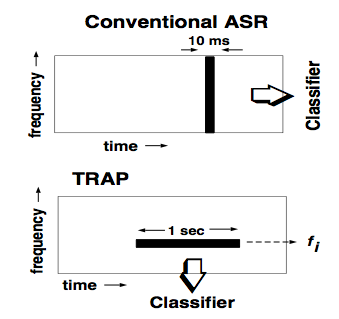
\includegraphics[width=.5\textwidth]{images/trap_temporal.png}}}
 \caption{The temporal paradigm for TRAP extraction versus conventional features (e.g. MFCC). \cite{traps1}}
 \label{fig:trap_temporal}
\end{figure}

\begin{figure}
	\begin{center}
		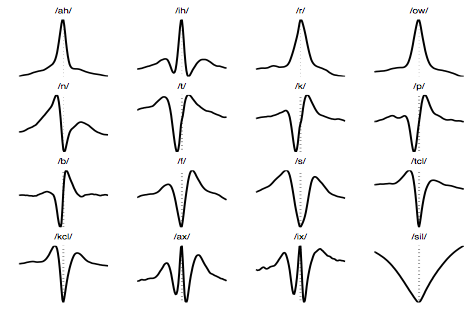
\includegraphics[width=1\textwidth]{images/phoneme_traps.png}
		\caption{Mean TRAPs of various phonemes in the 5th critical band. \cite{traps1}}
		\label{fig:phoneme_traps}
	\end{center}
\end{figure}

\begin{figure}
 \centerline{\framebox{
 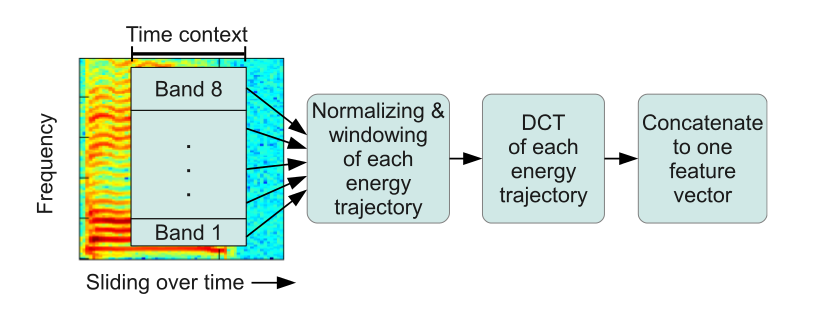
\includegraphics[width=\columnwidth]{images/trap_extraction.png}}}
 \caption{TRAP extraction process. \cite{jens}}
 \label{fig:traps}
\end{figure}




\section{Distance calculation} \label{sec:tech_distances}
In this section, two algorithms for distance calculation used in this work are described. Dynamic Time Warping (DTW) is used for calculating optimal alignments between two sequences of continuous values, while Levenshtein alignment is particularly useful for finding the optimal alignment (and therefore the minimum distance) between two sequences with discrete values, such as character strings, when allowing deletions, insertions, and replacements.

\subsection{Dynamic Time Warping}
Dynamic Time Warping (DTW) is an algorithm for finding an optimal alignment between two time sequences of vectors $X$ and $Y$, which was originally developed for aligning speech sequences to each other \cite{rabiner}. $X$ and $Y$ are not required to have the same length (i.e. $X = (x_1,...,x_M$) and $Y = (y_1,...,y_N) $). To this end, varying durations of parts of each sequence are allowed. The result is a warping path $W = w_1,...,w_K$ where each element represents an alignment of the elements of the two sequences (i.e. $w_k = (m_k,n_k)$ represents the alignment of the elements $x_{m_k}$ and $y_{n_k}$ of $X$ and $Y$).\\
In classical DTW, the warping path must fulfill three restrictions:
\begin{description}
	\item[1. Boundary condition] The warping path must align the whole sequences to each other - i.e. $w_1 = (1,1)$ and $w_K = (M,N)$.
	\item[2. Step size condition] The warping path may only step sequentially forward in either direction - i.e. $w_{k+1} - w_k \in \{(0,1),(1,0),(1,1)\}$. 
	\item[3. Monotonicity condition] The warping path cannot skip backwards - i.e. $m_1 \leq m_2 \leq ... \leq m_K$ and $n_1 \leq n_2 \leq ... \leq n_K$. (This is, in fact, already implied by condition 2).
\end{description}
A graphic example of such an alignment is given in figure \ref{fig:dtw_example}.\\

\begin{figure}
	\begin{center}
		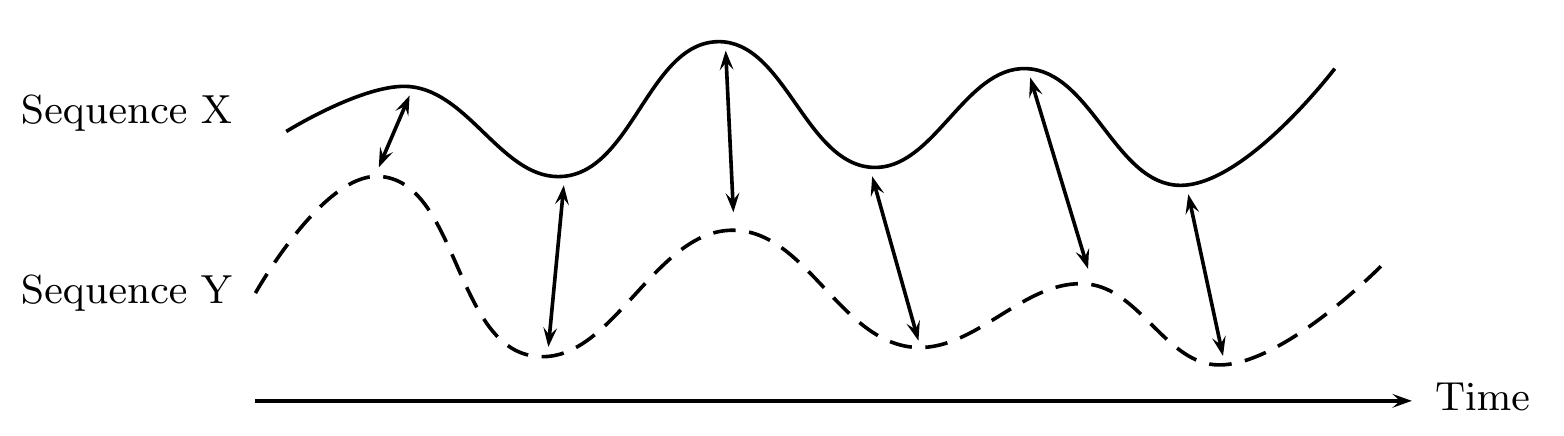
\includegraphics[width=1\textwidth]{images/dtw_example.png}
		\caption{Example of a DTW alignment. Alignment between points is represented by the arrows. \cite{meinard_retrieval}}
		\label{fig:dtw_example}
	\end{center}
\end{figure}

A DTW consists of two steps: Cost calculation and path detection. In the cost calculation steps, a local cost $c$ is calculated for all pairs $(x_m, y_n)$, resulting in a cost matrix $C$. An example is shown in figure \ref{fig:dtw_cost}. Common cost functions include the Manhattan distance and the cosine distance (i.e. the complement of the normalized inner product), which was used in this work:
\begin{equation}
c(x_m,y_n) =  1 - cos(\theta)
\end{equation}
where $\theta$ is the angle between $x_m$ and $y_n$.\\

In the second step, an optimal warping path is calculated on the cost matrix. The cost of a warping path is
\begin{equation}
c_W(X,Y) =  \sum_{k=1}^{K} c(x_{m_k}, y_{n_k})
\end{equation}
and the optimal warping path is the one with minimal cost - i.e. the DTW cost:
\begin{equation}
DTW(X,Y) =  \min\{c_W(X,Y)|W \text{ is a warping path}\}
\end{equation}

Consequently, the DTW cost can also be used to compare the quality of alignments of one query sequence to multiple other sequences when taking the varying lengths into account.
%TODO: hier beschreiben?
The path calculation is commonly solved using a Dynamic Programming algorithm \cite{meinard_retrieval}. In this work, the implementation from \cite{ellis_dtw} is used.\\

Subsequence DTW is a variant of this algorithm in which the boundary condition is loosened. This means that the optimal warping path can run along a subsequence of the longer compared sequence instead of the full series. This is more computationally expensive since more paths need to be calculated for comparison.

\begin{figure}
	\begin{center}
		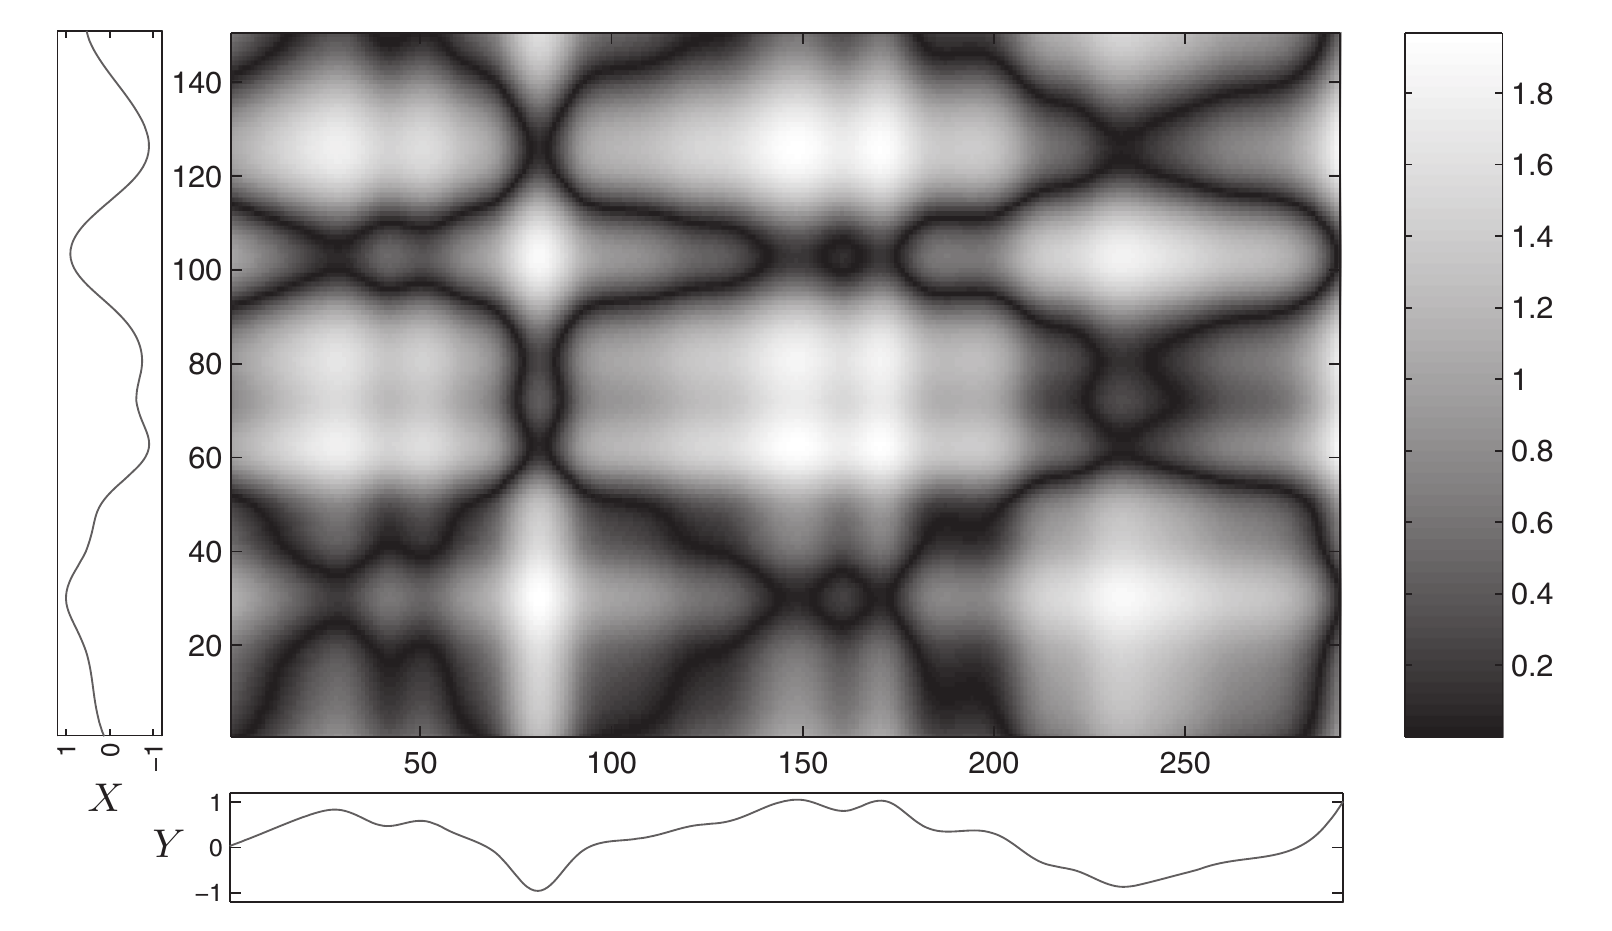
\includegraphics[width=0.8\textwidth]{images/dtw_cost.png}
		\caption{Example of a matrix of costs between two sequences $X$ and $Y$ using the Manhattan distance as the local cost measure. \cite{meinard_retrieval}}
			\label{fig:dtw_cost}
		\end{center}
	\end{figure}


\subsection{Levenshtein distance}
The Levenshtein distance, also called edit distance, is a measure of similarity between two strings (or character sequences). The algorithm was first described by Levenshtein in 1965 \cite{levenshtein} and can also be used to retrieve an optimal alignment (so-called approximate string matching \cite{navarro}). In that sense, it serves a similar purpose as DTW for strings instead of time sequences. This measure is commonly used in the fields of Computational Biology, Natural Language Processing, and signal processing.\\

The distance is the sum of character operations necessary to transform one string into the other. These operations can be substitutions, insertions, or deletions, which may be weighted differently. An example is shown in figure \ref{fig:levenshtein_example}. If each operation has a cost of 1, the Levenshtein distance in this example is 5; if substitutions are weighted with a cost of 2, the distance is 8.\\

Just like DTW, this problem is usually solved efficiently with a Dynamic Programming approach. For two strings $X = (x_1,x_2,...,x_M)$ and $Y = (y_1,y_2,...,y_N)$, the initial step is then defined as
\begin{equation}
L(0,0) = 0 , L(i,0) = \sum_{k=1}^{i} I(x_k) , L(0,j) = \sum_{k=1}^{j} D(y_k)
\end{equation}
and the recursive step is defined as
\begin{equation}
L(i,j) = \min \begin{cases}
L(i-1,j) + D(y_j)\\
L(i,j-1) + I(x_i)\\
L(i-1,j-1) + S(x_i,y_j)
\end{cases}       
\end{equation}
where $L(i,j)$ is the Levenshtein distance at step $(i,j)$ and $D$, $I$, and $S$ are the costs for deletions, insertions, and substitutions respectively \cite{applied_computing}. The over-all Levenshtein distance is $L(M,N)$.

\begin{figure}
	\begin{center}
		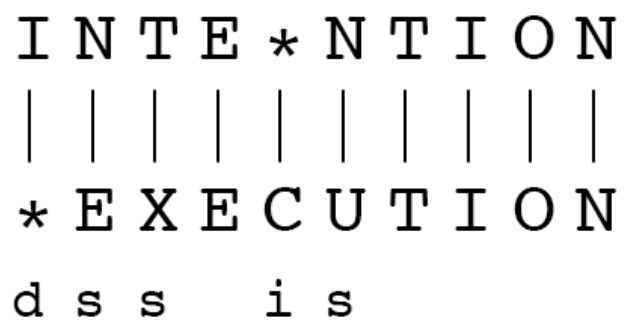
\includegraphics[width=0.4\textwidth]{images/levenshtein_example.png}
		\caption{Example of a Levenshtein distance calculation between the two strings ``INTENTION'' and ``EXECUTION''. Found operations (\textbf{d}eletions, \textbf{i}nsertions, \textbf{s}ubstitutions) are shown at the bottom. \cite{levenshtein_lecture}}
		\label{fig:levenshtein_example}
	\end{center}
\end{figure}




\section{Machine learning algorithms} \label{sec:tech_ml}
This section describes the various Machine Learning algorithms employed throughout this thesis. Gaussian Mixture Models (GMMs), Hidden Markov Models (HMMs), and Support Vector Machines (SVMs) are three traditional approaches that are used as the basis of many new approaches, and were used for several starting experiments. i-Vector processing is a relatively new, more sophisticated approach that bundles several other machine learning techniques.\\
In recent years, Deep Learning has become the standard for machine learning applications \cite{schmidhuber_dl}. This chapter also describes a new approach that was used extensively in this work: Deep Neural Networks (DNNs).



\subsection{Gaussian Mixture Models}
In their basic form, Gaussian Mixture Models (GMMs) are a form of unsupervised learning. Given a set of observations $X = (x_1, x_2, ..., x_N)$, their probability distribution is modeled with a superposition of Gaussian distributions:
\begin{equation}
p(x_n | \lambda ) = \sum_{i=1}^M p_i b_i(x)
\end{equation}
where $b_i$ are the constituting distributions, $p_i$ are the mixture weights, and $\lambda$ are the model parameters. A visualization is shown in figure \ref{fig:gmm_structure}. If the observations are multidimensional (which is the case for audio features), multivariate Gaussians (with $D$ dimensions) are used for this:
\begin{equation}
b_i(x) = \frac{1}{ (2\pi)^{D/2} \det(\Sigma_i)^{1/2}} \exp \left\{-\frac{1}{2} (x - \mu_i) \Sigma_i^{-1} (x - \mu_i) \right\}
\end{equation}
where $\mu_i$ is the mean vector and $\Sigma_i$ is the covariance matrix.\\
These parameters, together with the mixture weights, define the model:
\begin{equation}
\lambda = \left\{ p_i, \mu_i, \Sigma_i \right\}, i = 1,...,M
\end{equation}
For each observation $o_j$, the contribution of each Gaussian $b_i$ can be calculated as:
\begin{equation}
%???
p_{ni} = P(i | n) = \frac{b_i P(i)}{P(x_n)} 
\end{equation}
The overall likelihood of the model is:
\begin{equation}
L = \prod_{n=1}^N P(x_n)
\end{equation}

In order to find the optimal parameters $\lambda$, the iterative Expectation Maximization (EM) algorithm is commonly used \cite{dempster_laird}. In the expectation step, $L$ is calculated; in the maximization step, the parameters are adapted. This is repeated until convergence. An example of such a training procedure is visualized in figure \ref{fig:gmm_training}.\\

\begin{figure}
	\begin{center}
		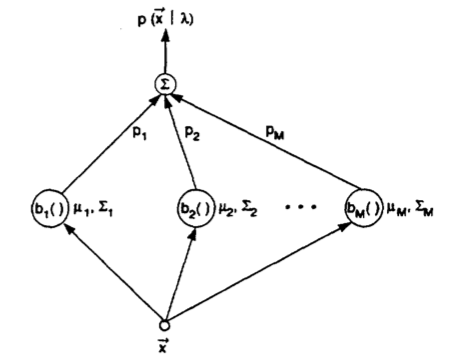
\includegraphics[width=0.7\textwidth]{images/gmm_structure.png}
		\caption{Visualization of a GMM. The Gaussian mixture is the weighted sum of several Gaussian distributions, where $p_i$ are the mixture weights and $b_i$ are the Gaussians. \cite{reynolds_rose}}
		\label{fig:gmm_structure}
	\end{center}
\end{figure}

\begin{figure}
	\begin{center}
		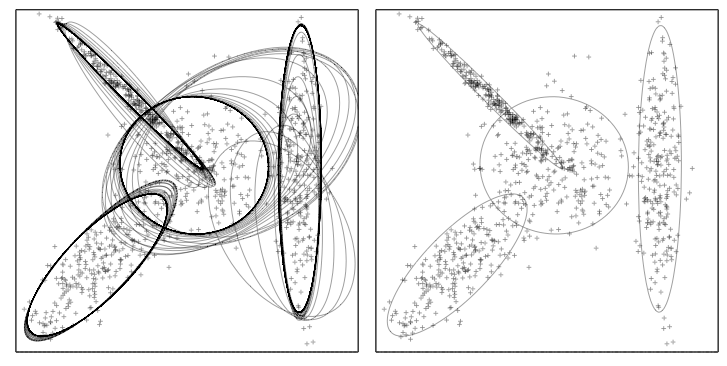
\includegraphics[width=1\textwidth]{images/gmm_training.png}
		\caption{Example of a GMM in two dimensions. Crosses signify the data points, ellipses the three multivariate Gaussians. On the left-hand side, the evolution of the estimated means and covariances of these Gaussians during the EM process is shown;  the right-hand side shows the converged mixture. \cite{numerical_recipes}}
		\label{fig:gmm_training}
	\end{center}
\end{figure}

Gaussian Mixture Models have been used in many areas of machine learning, for example in ASR \cite{reynolds_rose}, in image retrieval \cite{permuter}, in financial modeling \cite{alexander}, and in visual tracking \cite{chen_adebomi}. When used for classification, one GMM is trained for each class $S = (s_1, s_2, ..., s_J)$ separately, resulting in $J$ sets of parameters $\lambda$. The likelihood $L_j$ of each class is then determined, and the most likely class is chosen:
\begin{equation}
C = \argmax_{1 \leq j \leq J } P(\lambda_j | X) = \argmax_{1 \leq j \leq J} \frac{p(X | \lambda_j) P(\lambda_j)}{p(X)}
\end{equation}
(according to Bayes' rule). If all classes and all observations are equally likely, this simplifies to
\begin{equation}
C = \argmax_{1 \leq j \leq J } p(X | \lambda_j) 
\end{equation}
In practice, log-probabilities are commonly used for numerical reasons, resulting in the calculation:
\begin{equation}
C = \argmax_{1 \leq j \leq J} \sum_{n=1}^N p(x_n | \lambda_j)
\end{equation}

In addition to this direct use for classification, GMMs are often used to model the emission probabilities in Hidden Markov Models.



%256
%!
\subsection{Hidden Markov Models}
%!
% definition - statistical model of Markov processes - i.e. only depends on previous state
% presented by Baum
% good at modeling temporal processes; used in asr a lot (rabiner, young/gales)
% probabilities can be modeled in different ways (e.g. GMMs, DNNs), still tractable
% special cases: restrictions to transition matrix
%invariant to translation (bishop)
% components: hidden states -> observations , transitions (image)
% training: Baum-Welch (special case of EM) (and observation computation)
% hidden state estimation: Viterbi
% asr: hidden states phones, observations acoustic feature vectors; often left-to-right (non-ergodic)
Markov models are statistical models of Markov processes - i.e. sequences of states in which the probability of each state only depends on the previous one. In a Hidden Markov Model (HMM), these states are not directly observable, but may be inferred from the models emissions. HMMs were first suggested by Baum et al. around 1970 \cite{baum1}\cite{baum2}\cite{baum3}\cite{baum4}\cite{baum5}. Due to their ability to model temporal processes, they have been employed extensively in ASR \cite{rabiner_hmm1}\cite{rabiner_hmm2}\cite{jelinek}\cite{gales_young_hmm}. Apart from this field, they are also frequently used in Natural Language Processing \cite{manning_schuetze}, Optical Character Recognition \cite{nag}, and Computational Biology \cite{krogh}\cite{durbin}.\\

A HMM consists of four basic components:
\begin{itemize}
\item The observation (= emission) sequence $Y = (y_1, y_2, ..., y_T)$
\item The hidden state nodes $Q = (q_1, q_2, ..., q_N)$; the sequence of hidden states corresponding to the observation sequence will be denoted as $I = (i_1, i_2, ..., i_T)$ where $i_t \in Q$.
\item The transition probabilities between the hidden states, defined by a transition matrix $A \in \mathbb{R}^{N x N}$; additionally, the initial state distribution (i.e. the probability of starting in each state) $\pi \in \mathbb{R}^N$
\item The emission probabilities $B = (b_1(k), b_2(k), ..., b_N(k))$, mapping from the hidden states to the observations. These can, for example, be Gaussians for continuous outputs $y_t$, or conditional probabilities for discrete $y_t$.
\end{itemize}
The transition probabilities, initial state distribution, and emission probabilities define the model $\lambda$.\\

In the case of speech recognition, the observations are the feature vectors, and the hidden states are the phonemes generating these features. Such a model is visualized in figure \ref{fig:asr_hmm}. Different variants of HMMs can be created by restricting the transition matrix in certain ways; e.g., left-to-right HMMs, which only allow transitions to subsequent states and are often used in speech recognition and handwriting recognition \cite{bishop}. A particularly interesting property of HMMs for speech recognition is their relative invariance to warping along the time axis because states can usually be repeated for arbitrary amounts of time.\\

Three problems commonly need to be solved for problems modeled with HMMs: 
\begin{description}
\item[Evaluation] - i.e., how probable is an observation sequence given this model? In mathematical terms, the probability $P(Y, I | \lambda)$ is sought. The most straightforward way to do this would be to calculate this probability for each possible $Y$ of the length $T$ of the observation sequence, but this is very computationally expensive. For this reason, an algorithm called \textit{forward procedure} is used. A forward variable $\alpha$ representing the probability at time $t$ is introduced:
\begin{equation}
\alpha_t(i) = P(y_1, y_2, ..., y_t, i_t = q_i | \lambda )
\end{equation}
This can be solved inductively with the initialization
\begin{equation}
\alpha_1(i) = \pi_i b_i (Y_1), 1 \leq i \leq N
\end{equation}
and the induction step
\begin{equation}
\alpha_{t+1}(j) = \left[ \sum_{i=1}^N \alpha_t(i) a_ij \right] b_j (Y_{t+1})
\end{equation}
This is a form of Dynamic Programming.

\item[Training] - i.e., how can the parameters $\lambda$ be set optimally to maximize the probability of observed sequences? There is no analytical way to compute this, but the so-called \textit{Baum-Welch} algorithm (which is a special case of the Expectation Maximization algorithm) allows for an iterative estimation of the parameters. In order to do this, a backward variable $\beta$ is calculated analogous to $\alpha$ to represent the probability of the sequence from time $t+1$ to the end:
\begin{equation}
\beta_t(i) = P(y_{t+1}, y_{t+2}, ..., y_T, i_t = q_i | \lambda )
\end{equation}
\begin{equation}
\beta_T(i) = 1, 1 \leq i \leq N
\end{equation}
\begin{equation}
\beta_{t}(i) = \sum_{j=1}^N a_ij b_j (Y_{t+1})\beta_{t+1}(j)
\end{equation}

The probability of a path being in state $q_i$ at $t$ and making a transition to $q_j$ at $t+1$ is then:
\begin{equation}
\xi_{t}(i, j) = \frac{\alpha_t(i)a_ij b_j (Y_{t+1} \beta_{t+1}(j)}{P(Y|\lambda)}
\end{equation}
This can be used to calculate the expected numbers of transitions and emissions, which can be re-adapted with statistics from the observation sequences and used to adjust $\alpha$ and $\beta$. This process is repeated until convergence.

\item[Decoding] - i.e., given an observation sequence, what is the most probable underlying sequence of hidden states? This is particularly interesting for speech recognition since the interpretation here is the detection of the phonemes generating a series of feature vectors.\\

Again, this problem is broken down by first defining a variable for the probability of being in state $q_i$ at time $t$:
\begin{equation}
\gamma_t(i) = P(i_t = q_i | Y, \lambda )
\end{equation}
and therefore, the most likely state at $t$ is:
\begin{equation}
i_t = \argmax_{1 \leq i \leq N}[\gamma_t(i)], 1 \leq t \leq T
\end{equation}

Using the forward and backward variables, this can be expressed as
\begin{equation}
\gamma_t(i) = \frac{\alpha_t(i) \beta_t(i)}{P(Y |�\lambda)}
\end{equation}
This problem can be solved efficiently with the \textit{Viterbi algorithm}, which again employs Dynamic Programming.
\end{description}


\begin{figure}
	\begin{center}
		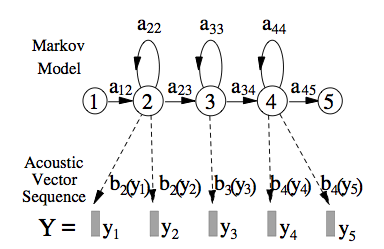
\includegraphics[width=0.6\textwidth]{images/asr_hmm.png}
		\caption{A HMM as it is commonly used in ASR, with phonemes as hidden states and acoustic feature vectors as the observations. $a_12, a_22, a_23,...$ are elements of the transition matrix $A$; $b_2(y1_), b_2(y_2), b_3(y_3)$ are elements of the output probability matrix $B$; $Y = y_1,y_2,...$ is the observation sequence. \cite{gales_young_hmm}}
		\label{fig:asr_hmm}
	\end{center}
\end{figure}

\subsection{Support Vector Machines}
%! clean up
Support Vector Machines (SVMs) are another type of supervised machine learning models, which are able to learn relationships between feature vectors $\textbf{x}_i \in \mathbb{R}^{n}$ and their expected classes $y_i, i=1,...,L$.
%In all supervised classification tasks, a training data set and a classification data set are provided. Each of these sets consists of previously extracted features of the training entities (or musical pieces in the case of genre classification) and, for the training data set, annotation labels (or genres in the case of genre classification). The training data set is denoted here as pairs of $\left(\mathbf{x}_{i}, y_{i}\right), i=1..l$, with $\textbf{x}_i \in \mathbb{R}^{n}$ being the feature vectors and $y_{i}$ being their assigned classes. The classifier tries to find similarities behind the training data for each label and separation conditions between the labels. With this information, the classifier is then able to assign a label to the classification data entities.\\
SVMs attempt to solve this problem by grouping the training data vectors $\mathbf{x}_{i}$ and finding separating (hyper-)planes (with the normal vector $\mathbf{w}$ and the offset $b$) between the points of the different classes (or annotation labels) $y_{i}$. In doing so, they try to maximize the margin between the plane and the data points. Additionally, the feature vectors may be transformed into a higher-dimensional space by the function $\phi(\textbf{x}_i)$ to make them more easily separable (as demonstrated in figure \ref{fig:svm_transformation}).\\

In \cite{techreport:practical_svm}, this training process is expressed (for a two-class problem) as:
\begin{equation}
\begin{aligned}
& \min\limits_{\mathbf{w},b,\xi} & & \frac{1}{2}\mathbf{w}^{T}\mathbf{w} + C \sum\limits_{i=1}^{l}\xi_{i} \\
& \text{subject to} & & y_{i}(\mathbf{w}^{T} \phi(\mathbf{x}_{i})+b) \geq 1-\xi_{i} , \\
&&& \xi_{i} \geq 0
\end{aligned}
\end{equation}
(with $\xi_{i}$ being a slack variable and $C > 0$ being a penalty parameter for the error term, higher $C$s allowing for fewer outliers (\cite{article:intro_svm}).
\begin{figure}[htbp]
	\centering
	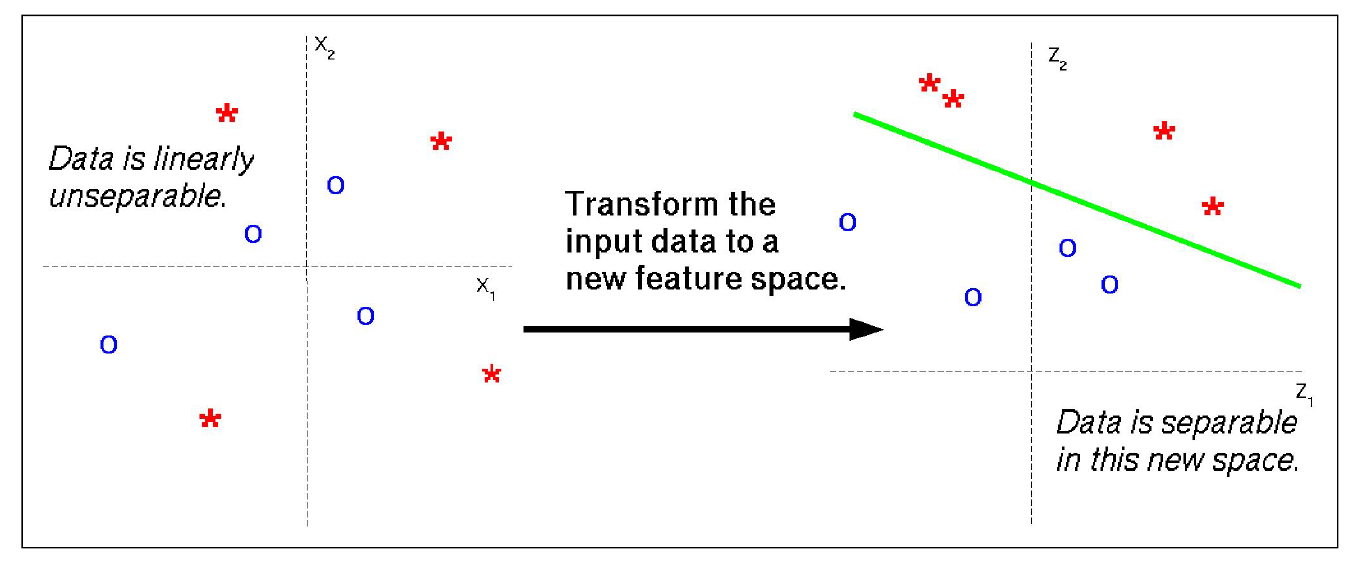
\includegraphics[width=0.9\textwidth]{images/svm_transformation.png}
	\caption{A set of data points which cannot be separated linearly in their original form (left), but can be separated after transformation into another space (right). \cite{article:intro_svm}}
	\label{fig:svm_transformation}
\end{figure}
\medskip
\\
$K(\mathbf{x}_{i},\mathbf{x}_{j}) \equiv \phi(\mathbf{x}_{i})^{T} \phi(\mathbf{x}_{j})$ is called a ``kernel function''. Several variants are possible, e.g. a linear kernel:
\begin{equation}
K(\mathbf{x}_{i},\mathbf{x}_{j}) = \mathbf{x}_{i}^{T}\mathbf{x}_{j}
\end{equation}
It is often useful to use a non-linear kernel because the data points may not be linearly separable (even after the transformation into a higher-dimensional space). An example is shown in figure \ref{fig:svm_kernels}. The Radial Basis Function (RBF) kernel is a popular one:
\begin{equation}
K(\mathbf{x}_{i},\mathbf{x}_{j}) = e^{-\gamma \parallel \mathbf{x}_{i} - \mathbf{x}_{j} \parallel^{2}}, \gamma > 0
\end{equation}
\begin{figure}[htbp]
	\centering
	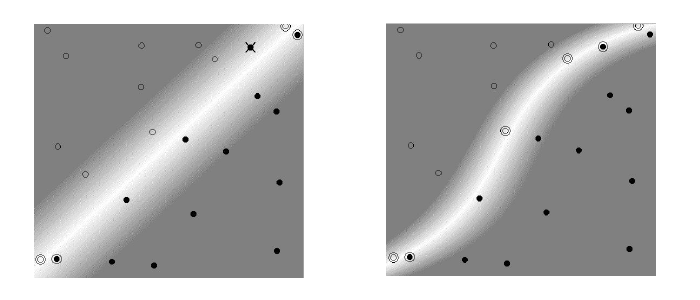
\includegraphics[width=0.9\textwidth]{images/svm_kernels.png}
	\caption{A set of data points which cannot be separated using a linear kernel (left), but can be separated with a polynomial kernel (right). \cite{article:svm_tutorial}}
	\label{fig:svm_kernels}
\end{figure}
\medskip
\\
As can be seen from the above equations, $C$ and $\gamma$ are free parameters. Their optimum values depend on the actual training data vectors. In \cite{techreport:practical_svm}, a grid search during each training is suggested to find them. 
\medskip
\\
The presented training process is useful for solving two-class problems. For multi-class problems, one-vs-one trainings for all combinations of classes are performed. Then, all of the developed classifiers are used for the classification of the evaluation data and a voting strategy is applied to determine the resulting class. 


\subsection{i-Vector processing}\label{subsec:tech_ivector}
i-Vector (identity vector) extraction was first introduced in \cite{Dehak2011}, and has since become a state-of-the-art technique for various speech processing tasks, such as speaker verification, speaker recognition, and language identification \cite{Martinez2011}. i-Vector extraction is not a stand-alone training algorithm, but rather a feature post-processing step using unsupervised machine learning. The resulting i-vectors for training examples are used to train other models (instead of the features themselves); during classification, i-vectors are extracted in the same way, and run through this model.\\
The main idea behind i-vectors is that all training examples (e.g. speech utterances) contain some common trends, which effectively add irrelevance to the data during training. Using i-vector extraction, this irrelevance can be filtered out, while only the unique parts of the data relevant to the task at hand remain. The dimensionality of the training data is massively reduced, which also makes the training less computationally expensive. As a side effect, all feature matrices are transformed into i-vectors of equal length, eliminating problems that are caused by varying utterance lengths.\\
Mathematically, this assumption can be expressed as:
\begin{equation}
M(u) = m+Tw
\end{equation}
where $M(u)$ is the GMM supervector for utterance $u$. The supervector approach was first presented in \cite{reynolds00} and has since been successfully applied to a number of speech recognition problems. A music example can be found in \cite{Charbuillet2011}. $m$ represents the language- and channel-independent component of $u$ and is estimated using a Universal Background Model (UBM). $T$ is a low-rank matrix modeling the relevant language- and channel-related variability, the so-called Total Variability Matrix. Finally, $w$ is a normally distributed latent variable vector: The i-vector for utterance $u$.\\

The following steps are necessary for i-vector extraction:
\begin{description}
\item[1. UBM training] A Universal Background Model (UBM) is trained using Gaussian Mixture Models (GMMs) from all utterances. This unsupervised model represents the characteristics that are common to all of them.
\item[2. Statistics extraction] 0th and 1st order Baum-Welch statistics are calculated for each of the utterances from the UBM according to:
\begin{equation}
N_c(u)=\sum_{t=1}^{L} P(c|y_t,\Omega)
\end{equation}
\begin{equation}
\widetilde{F_c}(u)=\sum_{t=1}^{L} P(c|y_t,\Omega)(y_t-m_c)
\end{equation}
where $u={y_1,y_2,...,y_L}$ denotes an utterance with $L$ frames, $c=1,...,C$ denotes the index of the Gaussian component, $\Omega$ denotes the UBM,  $m_c$ is the mean of the UBM mixture component $c$, and $P(c|y_t,\Omega)$ denotes the posterior probability that the frame $y_t$ was generated by mixture component $c$. As the equation shows, the 1st order statistics are centered around the mean of each mixture component.\\
\item[3. $T$ matrix training] Using the Baum-Welch statistics for all utterances, the Total Variability Matrix $T$ is now trained iteratively according to:
\begin{equation}\label{equ:trainT}
w = (I+T^t \Sigma^{-1} N (u) T)^{-1}T^t \Sigma^{-1} \widetilde{F}(u)
\end{equation}
using the Expectation Maximization algorithm.
\item[4. Actual i-vector extraction] Finally, an i-vector $w$ can be extracted for each utterance using equation \ref{equ:trainT} again. This can also be done for unseen utterances, using a previously trained $T$, and in this way be used during classification.
\end{description}

\subsection{Artificial Neural Networks}
Artificial Neural Networks have a long research history. Based on an idea by McCulloch and Pitts from 1943 \cite{mcculloch_pitts}, they were slowly developed into functional algorithms for classification and pattern recognition. Rosenblatt proposed a hardware design for a single-layer perceptron in 1958 \cite{rosenblatt}, while the first multi-layer networks were introduced by Ivakhnenko and Lapa in 1965 \cite{ivakhnenko}. In 1969, Minsky and Papert posited many practical limitations for Neural Networks \cite{minsky_papert}, which led to a decrease in interest.\\
The introduction of the backpropagation algorithm solved some of these issues and increased the training speed of multilayer networks \cite{werbos}, leading to a wider usage in speech recognition \cite{waibel_hanazawa} and other fields, such as computer vision \cite{srinivas} and Natural Language Processing \cite{goldberg}. However, other algorithms such as SVMs began to produce better results over time and thus overtook Neural Networks in popularity.\\
Over time, processing speed of computers increased, and better strategies and hardware for parallel computing became available. This the training of networks with many more layers possible, allowing for a much better adaptation to high-dimensional problems \cite{hinton_osindero}. Over the past 10 years, this so-called ``deep learning'' became the state of the art for many machine learning problems \cite{nytimes}\cite{schmidhuber_dl}\cite{deng_hinton_kingsbury}.\\

Artifical Neural Networks (ANNs) are inspired by ``real'' Neural Networks - i.e. the human brain and nervous system. They consist of neurons, which are nodes that can process inputs and send outputs, and the connections between them. These neurons are grouped in layers: An input layer, an output layer, and a number of hidden layers in between them. Historically, ANNs had no hidden layers at all; this type of ANN was called ``perceptron''. Later, hidden layers were introduced and the resulting networks were called ``Multilayer Perceptrons'' (MLPs).
%check this!
Networks with no hidden layers are only able to solve linear problems; the introduction of hidden layers added non-linear projections to the calculation. Recent ``Deep'' Neural Networks (DNNs) possess three or more hidden layers, leading to an exponential increase of the degrees of freedom and thus the possibility to model much more complex problems.\\

\begin{figure}[htbp]
	\centering
	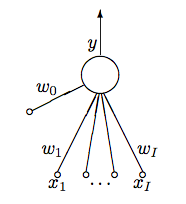
\includegraphics[width=0.3\textwidth]{images/neuron.png}
	\caption{Functionality of a single neuron in an ANN. The neuron computes a weighted sum of its inputs, and then applies an activation function, resulting in output $y$. \cite{mackay}}
	\label{fig:neuron}
\end{figure}


\begin{figure}
        \centering
        \begin{subfigure}[t]{0.3\textwidth}
		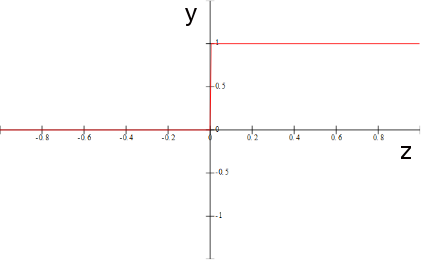
\includegraphics[width=\textwidth]{images/activation_heaviside.png}
                \caption{Heaviside binary step activation function}
                \label{fig:activation_heaviside}
        \end{subfigure}
                \begin{subfigure}[t]{0.3\textwidth}
		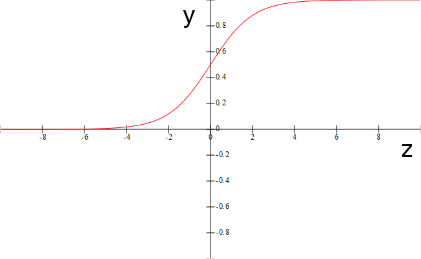
\includegraphics[width=\textwidth]{images/activation_sigmoid.png}
                \caption{Sigmoid activation function}
                \label{fig:activation_sigmoid}
        \end{subfigure}
                \begin{subfigure}[t]{0.3\textwidth}
		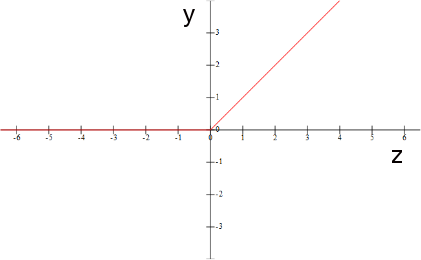
\includegraphics[width=\textwidth]{images/activation_relu.png}
                \caption{ReLU activation function}
                \label{fig:activation_relu}
        \end{subfigure}
        \caption{Activation functions used for ANN neurons. \cite{medium}}
          \end{figure}
          
   
The function of a single neuron is visualized in figure \ref{fig:neuron}. Classical neurons compute a weighted sum $z$ of their inputs $\textbf{x} = (x_1,x_2,...,x_I)$:
\begin{equation}
z = w_0 + \sum_{i=1}^I x_i w_i = w_0 + \textbf{w}^T \textbf{x}
\end{equation}
%check logit
where $\textbf{w} = (w_1,w_2,...,w_I)$ is a vector of weights, and $w_0$ is a constant bias. This result is often called the ``logit''. Then, a nonlinear activation function can be applied. In perceptrons, this was the Heaviside step function, shown in figure \ref{fig:activation_heaviside}, resulting in a binary output:
\begin{equation}
y = \begin{cases}
1 \text{ if } z \leq 0\\
0 \text{ otherwise}
\end{cases}       
\end{equation}
An activation function commonly used is the sigmoid function, shown in figure \ref{fig:activation_sigmoid}:
\begin{equation}
y = \frac{1}{1 + e^{-z}}
\end{equation}
Neurons of this type are called ``logistic'' neurons. This function is often applied because it generates a smooth, real-valued output and has easy-to-use derivatives, simplifying the training process.\\
Rectified linear units (ReLUs) are also used frequently since they train faster than logistic units and retain more information that is relevant in the middle layers (in particular, this is leads to sparsity for small inputs and a lower risk of vanishing or exploding gradients). The function is shown in figure \ref{fig:activation_relu}:
\begin{equation}
y = \max(0, z)
\end{equation}
In the last layer, a so-called softmax activation function is often applied. This function takes the outputs of all neurons into account, and computes a probability distribution (i.e. all the outputs will sum up to one and represent the likelihood of the corresponding class):
\begin{equation}
y_j = \frac{e^{z_j}}{\sum_{k=1}^M e^{z_k}}, 1 \leq j \leq M
\end{equation}
where $M$ is the number of output neurons.\\

\begin{figure}[htbp]
	\centering
	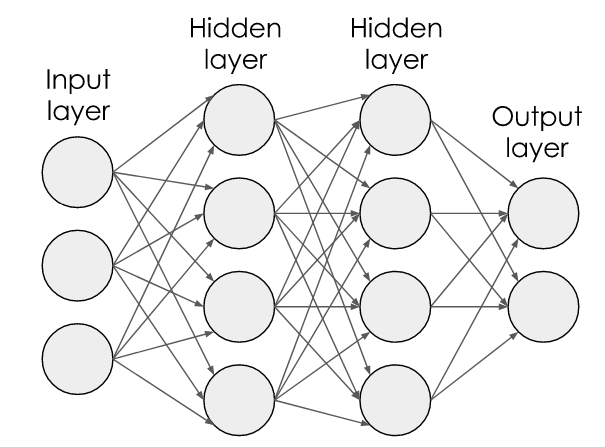
\includegraphics[width=0.4\textwidth]{images/feedforward.png}
	\caption{Schematic of a feed-forward neural network with an input layer with four neurons, two hidden layers with four neurons each, and an output layer with two neurons. \cite{medium}}
	\label{fig:feedforward}
\end{figure}
In addition to the various types of neurons, ANNs themselves can be grouped into different of types. In their basic configuration, ANNs will have multiple layers of the described neurons where connections are only allowed in one direction. A schematic is shown in figure \ref{fig:feedforward}. This type of network is called ``feed forward'' or, in the context of Deep Learning, a Deep Neural Network (DNN).\\
If connections that skip back are allowed in the network, the network is called a Recurrent Neural Network (RNN). These networks are particularly useful for modeling time-dependent series because they have the ability to ``store'' temporal states in their units. However, they were deemed impractical for a long time because they exhibit the exploding/vanishing gradient problem during training \cite{Hochreiter1998}. This problem was solved with the introduction of memory cells in place of neurons, in particular Long Short-Term Memory (LSTM) units \cite{Hochreiter1997} and Gated Recurrent Units (GRU) \cite{Cho2014}. Nowadays, RNNs are being used successfully in a number of research tasks \cite{lstm_sak_senior}.\\
A third type of Neural Network are Convolutional Neural Networks (CNNs). These networks add layers of filters (so-called convolutional layers) before or in between classical fully-connected layers. The parameters of these filters are trained jointly with the other layers. For this reason, CNNs are able to ``learn'' a feature representation of the input. They were first used in image recognition \cite{krizhevsky}, but are now also being used for audio-related tasks such as environmental sound classification \cite{piczak} and ASR \cite{abdelhamid}. A disadvantage of both RNNs and CNNs is the computational complexity of training them, and the requirement for even more training data because they possess even more degrees of freedom than DNNs of comparable sizes.\\
%woanders?
In this work, DNNs with logistic units in the hidden layers and a softmax output layer were used in phoneme classification tasks.\\

Neural Network training is performed via the backpropagation algorithm. This algorithm is based on the calculation of a cost (or error) function $E$, which computes the difference between the network output and the expected output (e.g. the annotated classes in the training data). Then, the partial derivatives of the cost are calculated with regards to the weights, using the outputs and logits for the chain rule:
\begin{equation}
\frac{\partial E}{\partial w_{ij}} = \frac{\partial E}{\partial y_j} \frac{\partial y_j}{\partial z_j} \frac{\partial z_j}{\partial w_{ij}}
\end{equation}
Then, the weights are adjusted accordingly:
\begin{equation}
\Delta w_{ij} = - \eta \frac{\partial E}{\partial w_{ij}}
\end{equation}
where $\eta$ is the so-called learning rate which must be chosen carefully to ensure convergence of the training process.\\
In the same way, the error is propagated further backwards through the model to adjust the weights of the previous layers. This is done until all the weights have been adjusted. Then, the next batch of training data is passed through the model and the process is repeated. The training process is performed until the weights converge (or until a fixed number of iterations has been reached).\\

A commonly used cost function is the squared error measure:
\begin{equation}
E_S = \frac{1}{2} \sum_{j=1}^{M} (t_j - y_j)^2
\end{equation}
where $t_j$ is the target value for output unit $j$. 
%The partial derivative for the output units is:
%\begin{equation}
%\frac{\partial E_S}{\partial y_j} = - (t_j - y_j)
%\end{equation}
%With regards to the weights:
%\begin{equation}
%\frac{\partial E_S}{\partial w_ij} = \frac{\partial E}{\partial y_j} \frac{\partial y_j}{\partial z_j} \frac{\partial z_j}{\partial w_ij} = 
%\end{equation}


Alternatively, the cross-entropy is often chosen as the cost function when using a softmax output layer:
\begin{equation}
E_C = - \sum_{j=1}^M t_j \log y_j
\end{equation}
%\begin{equation}
%\frac{\partial C}{\partial z_i} = \sum_{j=1}^M \frac{\partial C}{\partial y_j} \frac{\partial y_j}{\partial z_i} = y_i - t_i
%\end{equation}
\\
One of the major issues in Neural Networks is that of overfitting: The model adapts too well to the training data and is not able to sufficiently generalize to new data anymore. (In extreme cases, the model simply learns all the training data by heart). This is especially relevant for deep networks because of the many degrees of freedom.\\
There are several strategies to overcome this problem. One of the most frequently used regularization techniques is dropout: During training, nodes in the network are deactivated randomly, effectively resulting in many different network structures and making the whole network robust to variations in the data. The most crucial point, however, is the amount of data used for training the network. The more variety is available, the lower the risk of overtraining.\\
The so-called ``curse of dimensionality'' is a concept that applies to many machine learning algorithms:
However, Goodfellow et al. make an argument that Deep models operate on a different level altogether \cite{goodfellow}: Where traditional machine learning methods make an assumption of smoothness of the hidden functions to be represented, deep models actually attempt to model the underlying structures in a distributed way. This means that information about outputs can be learned in a shared way - i.e., if two classes have something in common, the model is also able to represent this fact. Practically, the many degrees of freedom do not lead to ``learning by heart'', but instead allow for an internal representation of highly complex relationships. Goodfellow et al. mention two interpretations of the deep modeling capabilities: Learning a representation composed of simpler representations (e.g. corners defined by edges), or learning sequential step that build on top of each other (e.g. first locate objects, then segment them, then recognize them). There is also a number of publications that demonstrate better generalization abilities for deeper networks \cite{bengio07}\cite{bengio09}\cite{ciresan}\cite{erhan09}\cite{krizhevsky}\cite{szegedy}. In an experiment in \cite{goodfellow_experiment}, shallow models with three hidden layers overfit at 20 million parameters, while a deep model (11 hidden layers) benefits from more than 60 million. This is because a deep model has the capability to learn the actual explanatory factors behind the expected outputs (e.g. learning about different genders or whether a person is wearing glasses when modeling faces \cite{radford}).

%!!! hier weiter mit CoD - Goodfellow
%particularly when seen as feature learning... - non-linear mapping; or representing different features of the input (faces: male vs. female, glasses...)
% empirical proof
%also search for degrees of freedom

%structure
%types - dnn, cnn, rnn; types of neurons - relu, sigmoid; softmax for cfy
%training, backprop
% problems: overtraining -> CoD



%
%\section{Evaluation}
%\subsection{Evaluation of phoneme recognition and alignment tasks}
%%alignment? - duration acc. - no, mean error
%\subsection{Evaluation of language identification tasks}
%\subsection{Evaluation of keyword spotting tasks}

\section{Speech recognition systems and their evaluation} \label{sec:tech_systems}

\subsection{Phoneme recognition}\label{subsec:tech_systems_phonerec}
In common ASR systems, phoneme recognition is performed by training an acoustic model that is able to determine the probability of phoneme occurrences in unseen audio frames. The result of this is a so-called phoneme posteriorgram - i.e. a matrix of the probabilities of each possible phoneme over time. In a second step, another model is applied to this posteriorgram, taking into account the probabilities of phoneme sequences and words formed by these phonemes, and thus generating a phoneme string from the posterior probabilities. This step is called language modeling.\\

Language modeling is a field of research unto itself, and is a complex tasks for lyrics. For this reason, this work focuses on improving the acoustic modeling step. The training process is performed according to the general schema described in section \ref{sec:tech_general}. The specific adaptations are shown in figures \ref{fig:process_training_phones} and \ref{fig:process_classification_phones}: In training, phoneme annotations are used to defined the possible classes. A set of around 39 phonemes is common; the phoneme set used in this work is the one used in CMU Sphinx\footnote{\url{http://cmusphinx.sourceforge.net/}} and is listed with examples in appendix \ref{app:phonemes}. The used data sets contain annotations of monophones. In ASR, splitting phonemes into three temporal phases is common, resulting in so-called senones. This was also tested as described in section \ref{sec:phonerec_acap}.\\

\begin{figure}
	\begin{center}
		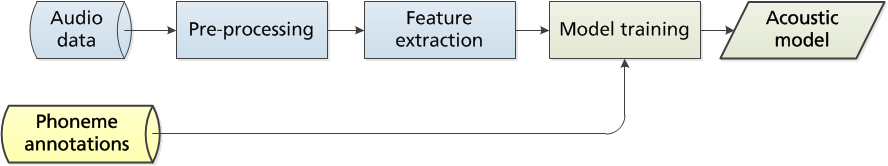
\includegraphics[width=1\textwidth]{images/process_training_phones.png}
		\caption{Schematic of the training procedure for phoneme recognition.}
		\label{fig:process_training_phones}
	\end{center}
\end{figure}
\begin{figure}
	\begin{center}
		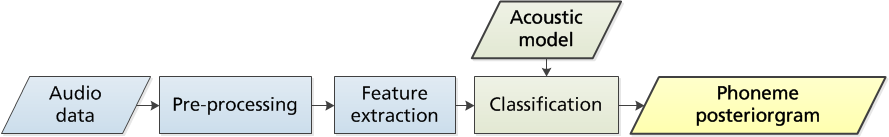
\includegraphics[width=1\textwidth]{images/process_classification_phones.png}
		\caption{Schematic of the classification procedure for phoneme recognition.}
		\label{fig:process_classification_phones}
	\end{center}
\end{figure}

 The whole training process then results in an acoustic model, which can be used for classification as shown in figure \ref{fig:process_classification_phones}. As described, classification results in a phoneme posteriorgram. An example is shown in figure \ref{fig:posteriorgram}. The time resolution of the posteriograms in this work is 10ms. Instead of language modeling, many of the following tasks build directly on the posteriogram. For evaluation of the phoneme recognition itself, Viterbi decoding with evenly weighted transitions is performed on the posteriorgrams. Then, the Phoneme Error Rate (PER) and the Weighted Phoneme Error Rate (WPER) are used for assessing the quality. The Phoneme Error Rate is simply the Levenshtein distance between the generated and the expected phoneme sequence where insertions, deletions, and replacements are weighted equally, normalized by the length of the expected sequence:
  \begin{equation}
    PER = \frac{D + I + S}{N}
 \end{equation} 
 where $D$ are deletions, $I$ are insertions, and $S$ are substitutions of phonemes and $N$ is the length of the sequence. (The accuracy measure used in some of the state-of-the-art works is the same as $1-PER$).\\
Some works also use a measure called $correct$, which ignores insertions. This makes sense if it is assumed that the phoneme results are used afterwards by an algorithm that is tolerant to insertions. In many cases, such post-processing steps will then also be tolerant to deletions. For cases like this, Hunt suggested a weighted error rate that punishes insertions and deletions less heavily than substitutions \cite{hunt}:
 \begin{equation}
    Weighted\ PER = \frac{0.5 D + 0.5 I + S}{N}
 \end{equation}  
 
 \begin{figure}
	\begin{center}
		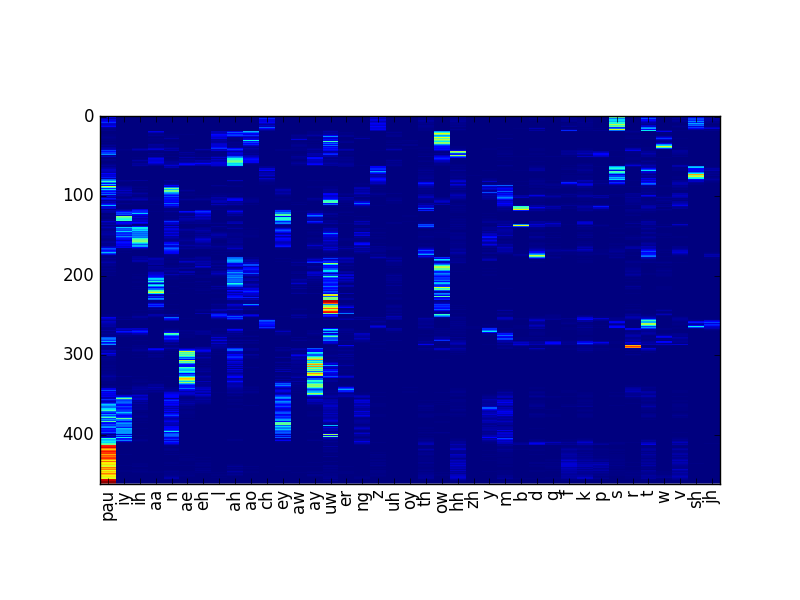
\includegraphics[width=1\textwidth]{images/posteriorgram.png}
		\caption{Example of a phoneme posteriorgram, the result of classification with an acoustic model. The posteriorgram represents the posterior probabilities of each phoneme over time. The time resolution in this example is 10ms.}
		\label{fig:posteriorgram}
	\end{center}
\end{figure}


\subsection{Language identification}
\begin{figure}
	\begin{center}
		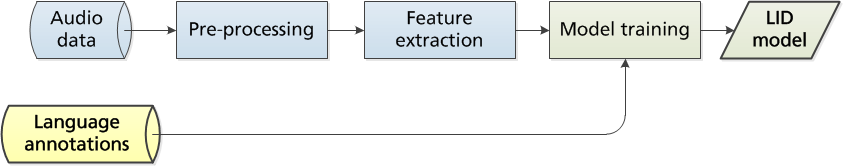
\includegraphics[width=1\textwidth]{images/process_training_lid.png}
		\caption{Schematic of the training procedure for language identification.}
		\label{fig:process_training_lid}
	\end{center}
\end{figure}
\begin{figure}
	\begin{center}
		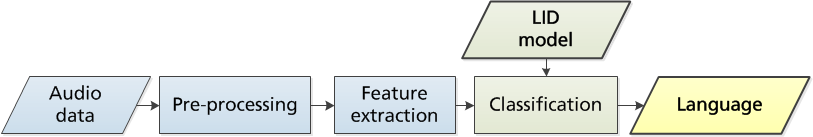
\includegraphics[width=1\textwidth]{images/process_classification_lid.png}
		\caption{Schematic of the classification procedure for language identification.}
		\label{fig:process_classification_lid}
	\end{center}
\end{figure}

Language identification has been extensively researched in the field of Automatic Speech Recognition since the 1980's. A number of successful algorithms has been developed over the years. An overview over the fundamental techniques is given by Zissman in \cite{zissman}.\\
Fundamentally, four properties of languages can be used to discriminate between them:
\begin{description}
	\item[Phonetics] The unique sounds that are used in a given language.
	\item[Phonotactics] The probabilities of certain phonemes and phoneme sequences.
	\item[Prosody] The ``melody'' of the spoken language.
	\item[Vocabulary] The possible words made up by the phonemes and the probabilities of certain combinations of words.
\end{description}
Even modern systems mostly focus on phonetics and phonotactics as the distinguishing factors between languages. Vocabulary is sometimes exploited in the shape of language models.\\
In ASR, the standard technique for language identification is Parallel Phone Recognition followed by Language Modeling (PPRLM). In this approach, acoustic and language models are trained for each language (or, in some cases, only the language models are different and just one acoustic model is used) . Unseen examples are then run through each model or combinations thereof, and the result with the highest likelihood determines the language (e.g. \cite{lid_li_ma} and \cite{lid_matejka}).\\
Other approaches directly train models for each language on the feature vectors (e.g. GMMs). This technique can be considered a ``bag of frames'' approach, i.e. the single data frames are considered to be statistically independent of each other. The trained models then describe probability densities for certain acoustic characteristics of each language. GMM approaches used to perform worse than their PPRLM counterparts, but the development of new features has made the difference negligible \cite{singer}. They are, in general, easier to implement since only audio examples and their language annotations are required. Allen et al. \cite{allen} report results of up to $76.4\%$ accuracy for ten languages. Different backend classifiers, such as Multi-Layer Perceptrons (MLPs) and Support Vector Machines (SVMs) \cite{campbell}, have also been used successfully instead of GMMs.\\
%HERE??
In this work, an approach that trains directly on the acoustic characteristics using i-vector extraction and SVMs is presented. The modifications to the general processing chain are presented in figures \ref{fig:process_training_lid} and \ref{fig:process_classification_lid}.\\
 
Additionally, a second approach based on phoneme posteriorgrams is tested. Statistics from the posteriorgrams are calculated, and then a second model is trained on these. Similar methods have been developed in ASR: Berkling presented an approach that uses sequences of recognized phonemes to discriminate between two languages (English and German), either with statistical modeling or with Neural Networks \cite{phdthesis:berkling_phd}. Mean errors of $0.12$ and $0.07$ on unseen data are achieved for the statistical approach and the Neural Network approach respectively when enough training data is available.\\
Li, Ma, and Lee present a system where acoustic inputs are tokenized into acoustic words, which do not necessarily correspond to phonetic n-grams. Then, language classifiers are trained on statistics of the acoustic words \cite{lid_li_ma_lee}. They obtain an equal error rate of $0.05$ for six languages using a universal phoneme recognizer for tokenization and SVMs for backend language recognition. Peche et al. \cite{peche} attempt a similar approach on languages with limited resources. The performance remains good even when only acoustic models trained on different languages are used.\\
In all of these approaches, tokenization of some sort is performed using the acoustic models. Since phoneme recognition on singing still performs relatively badly, statistics are calculated directly on the phoneme posteriors in this work\\.


For evaluation, all test examples are classified into exactly one language class. Then, the accuracy (i.e. the average retrieval) is calculated:
 \begin{equation}
    Accuracy = \frac{TP}{N}
 \end{equation}  
 where $TP$ are the True Positives, and $N$ is the number of all documents. In ASR, the average cost measure as recommended in \cite{nist_cavg} is also used widely now; however, to remain in line with other sung language identification approaches such as those described in chapter \ref{chap:sota}, the accuracy was still used in this work.

\subsection{Keyword spotting}\label{subsec:tech_kws}
In \cite{kws_overview}, three basic principles for keyword spotting in speech are mentioned:
\begin{description}
\item[LVCSR-based keyword spotting] {In this approach, a full transcription of the audio recording is performed using Large-Vocabulary Continuous Speech Recognition (LVCSR), which can then be searched for the keyword. 
%Both acoustic models and language models are employed for this step. The resulting text can then be searched for the requested keywords. 
This is expensive to implement and offers no tolerance for transcription errors - if the keyword is not transcribed correctly, it will never be found later.}
\item[Acoustic keyword spotting] {
%In contrast to the LVCSR approach, no full transcription is performed here. 
Acoustic KWS algorithms only search for the keyword on the basis of its acoustic properties. %This is commonly done with Hidden Markov Models (HMMs) and can either be performed directly on the audio or feature data, or on phoneme posteriorgrams obtained from an acoustic model.\\
This approach is easy to implement and provides some tolerance for pronunciation variations. However, it does not take any a-priori knowledge about the language into account (e.g. about plausible word or phoneme sequences).}
\item[Phonetic search keyword spotting]{
%Just like in LVCSR-based keyword spotting, 
Again, a full transcription of the audio recording is performed, but the full lattices are retained instead of just the final transcription. A phonetic search for the keyword can then be run on these lattices. This approach combines the a-priori knowledge of the LVCSR-based approach with the robustness of the acoustic approach.}
\end{description}

As described in the next chapter (section \ref{sec:sota_speechtosinging}), there are significant differences between speech and singing signals, which means that ASR approaches for keyword spotting cannot simply be transferred to singing. In particular, both LVCSR-based keyword spotting and Phonetic search keyword spotting depend heavily on predictable phoneme durations (within certain limits). When a certain word is pronounced, its phonemes will usually have approximately the same duration across speakers. The language model employed in both approaches will take this information into account. However, phoneme durations in singing are not as predictable in speech, as figure \ref{fig:phoneme_stats} demonstrates. For this reason, a simpler acoustic approach using keyword-filler HMMs is employed in this work.\\
Keyword-filler HMMs have been described in \cite{szoeke} and \cite{jansen}. In general, two separate HMMs are created: One for the requested keyword, and one for all non-keyword regions (=filler). The keyword HMM has a simple left-to-right topology with one state per keyword phoneme, while the filler HMM is a fully connected loop of states for all phonemes. These two HMMs are then joined. Using this composite HMM, Viterbi decoding is performed on the phoneme posteriorgrams. Whenever the Viterbi path passes through the keyword HMM, the keyword is detected. The likelihood of this path can then be compared to an alternative path through the filler HMM, resulting in a detection score. A threshold can be employed to only return highly scored occurrences. Additionally, the parameter $\beta$ can be tuned to adjust the model. It determines the likelihood of transitioning from the filler HMM to the keyword HMM. The whole process is illustrated in figure \ref{fig:kf_hmm}.

\begin{figure}
 \centerline{\framebox{
 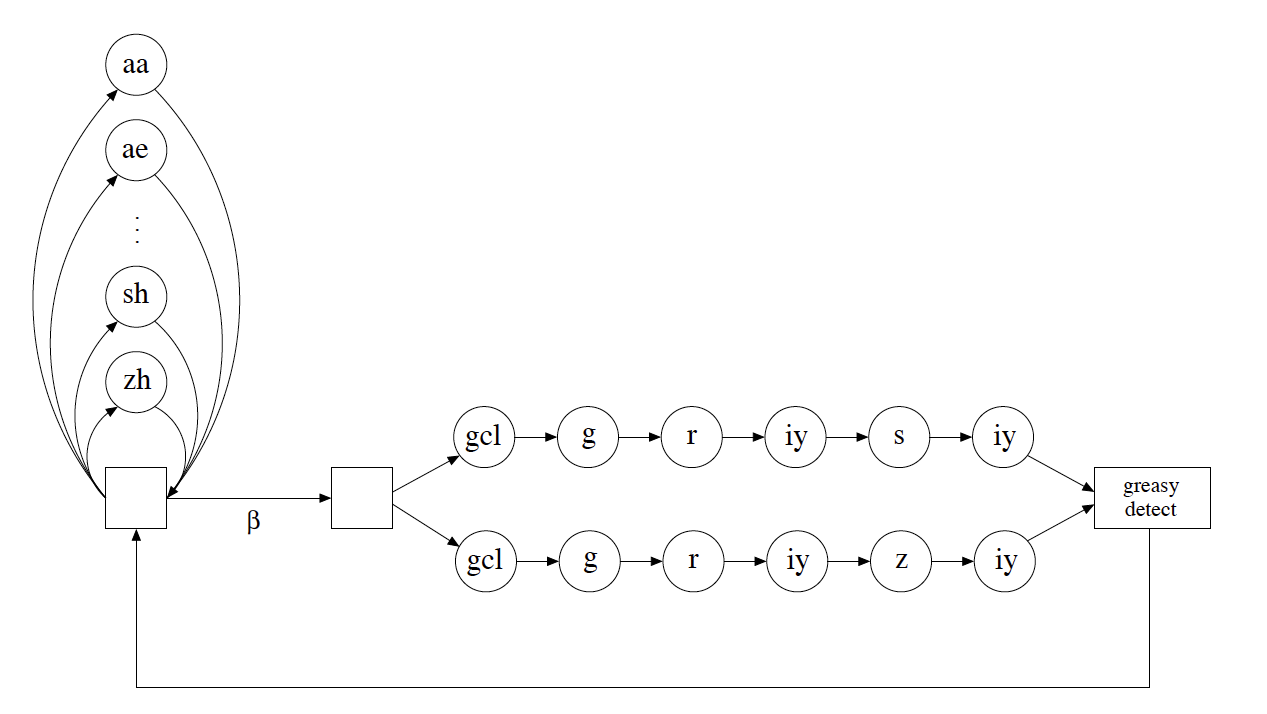
\includegraphics[width=.8\textwidth]{images/kw_filler_hmm.png}}}
 \caption{Keyword-filler HMM for the keyword ``greasy" with filler path on the left hand side and two possible keyword pronunciation paths on the right hand side. The parameter $\beta$ determines the transition probability between the filler HMM and the keyword HMM. \cite{jansen}}
 \label{fig:kf_hmm}
\end{figure}
Integration with the phoneme recognition system is shown in figure \ref{fig:process_training_kws}. Effectively, the keyword-filler HMM is added as a post-processing step after classification, and thus performed on the posteriorgrams.
\begin{figure}
	\begin{center}
		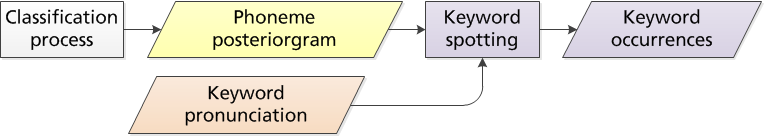
\includegraphics[width=0.8\textwidth]{images/process_classification_kws.png}
		\caption{Schematic of the procedure for keyword spotting.}
		\label{fig:process_training_kws}
	\end{center}
\end{figure}

Keyword spotting results are considered correct when they are detected within the expected songs, and are evaluated according to the $F_1$ measure. This measure is the harmonic mean of precision $P$ and recall $R$:
 \begin{equation}
    F_1 = 2 \frac{P \cdot R}{P + R}
 \end{equation}  
This measure is especially suited for cases where the classes are not balanced; in keyword spotting, occurrence of a keyword is much rarer than non-occurrence. In continuous speech recognition, the Figure Of Merit measure is often used \cite{fom}; however, since timing is not an issue in many applications for sung keyword spotting, this measure is not employed here.

\subsection{Alignment and retrieval}
\begin{figure}
	\begin{center}
		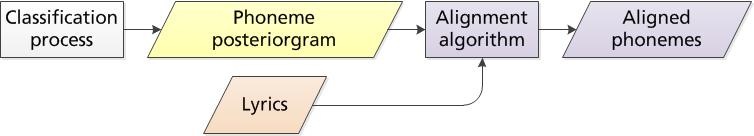
\includegraphics[width=0.8\textwidth]{images/process_classification_alignment.png}
		\caption{Schematic of the procedure for lyrics-to-audio alignment.}
		\label{fig:process_alignment}
	\end{center}
\end{figure}
Alignment is also performed on the phoneme posteriorgram. The lyrics with their phonetic pronunciation must be known in advance; then, an algorithm finds the best positions of each phoneme in the sequence in the posteriorgram. Traditionally, Viterbi decoding is used for this, with the transition matrix shaped such that only transitions through the expected phonemes are possible. In this work, two other methods (based on DTW and the Levenshtein distance) are also tested. The general process is shown in figure \ref{fig:process_alignment}.\\

For evaluation, the alignment approaches were submitted to the \textit{MIREX} 2017 challenge for lyrics-to-audio alignment\footnote{\url{http://www.music-ir.org/mirex/wiki/2017:Automatic_Lyrics-to-Audio_Alignment}}. In this challenge, the mean absolute error in seconds was used as the evaluation measure. For its calculation, all absolute deviations between the expected phoneme start and end timestamps and the automatically detected ones are calculated, averaged over the whole song, and once again over all songs. The measure was suggested in \cite{mesaros_alignment}.\\

\begin{figure}
	\begin{center}
		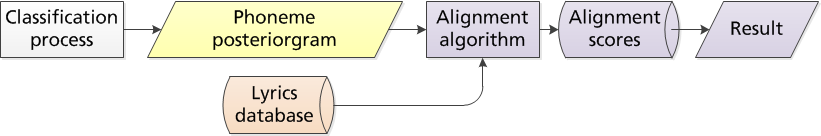
\includegraphics[width=0.9\textwidth]{images/process_retrieval.png}
		\caption{Schematic of the procedure for lyrics retrieval.}
		\label{fig:process_retrieval}
	\end{center}
\end{figure}
Lyrics retrieval can be interpreted as an alignment task as well. As shown in figure \ref{fig:process_retrieval}, alignment is performed on a whole database of lyrics instead of just those for a single song. Then, the scores for each alignment are compared, and the highest one determines the best match.\\

For evaluation, the accuracy when taking the first $N$ number of results into account (also called recognition rate in the state of the art) is calculated. For clarification: The first $N$ results are checked for occurrence of the expected result; then, the percentage of queries for which the correct result was detected is calculated. An alternative measure for tasks like this is the Mean Reciprocal Rank (i.e. the average inverse of the position where the expected result occurs); once again, the previously described measure was used for comparability with the state of the art.

